\documentclass{../template/myrpt}
\ExamName{非良导体导热系数的测量}

\begin{document}
\maketitle

\section{实验目的}
\begin{enumerate}[label=\arabic*. ]
  \item 了解热传导现象、热传导定律和导热系数的物理意义；
  \item 学习用稳态法测量非良导体导热系数的基本思路，体会参量转换法在实验设计中的作用；
  \item 掌握利用散热盘冷却速率间接求取样品导热系数的方法。
\end{enumerate}

\section{实验仪器}

\begin{figure}[htbp]
  \centering
  \begin{minipage}[c]{0.37\linewidth}
    \centering
    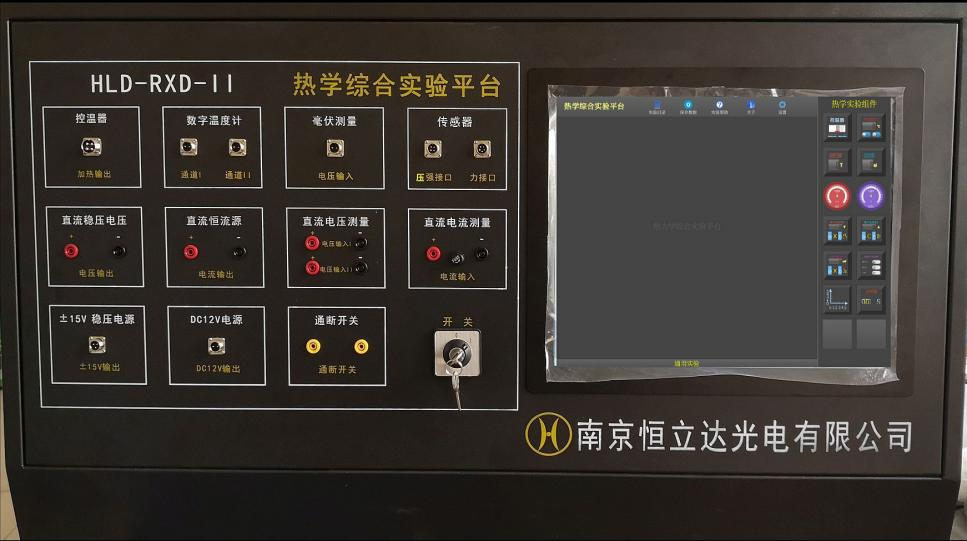
\includegraphics[width=\linewidth]{assets/image2.jpeg}
    \caption{热学综合实验平台}
  \end{minipage}
  \hspace{1em}
  \begin{minipage}[c]{0.47\linewidth}
    \centering
    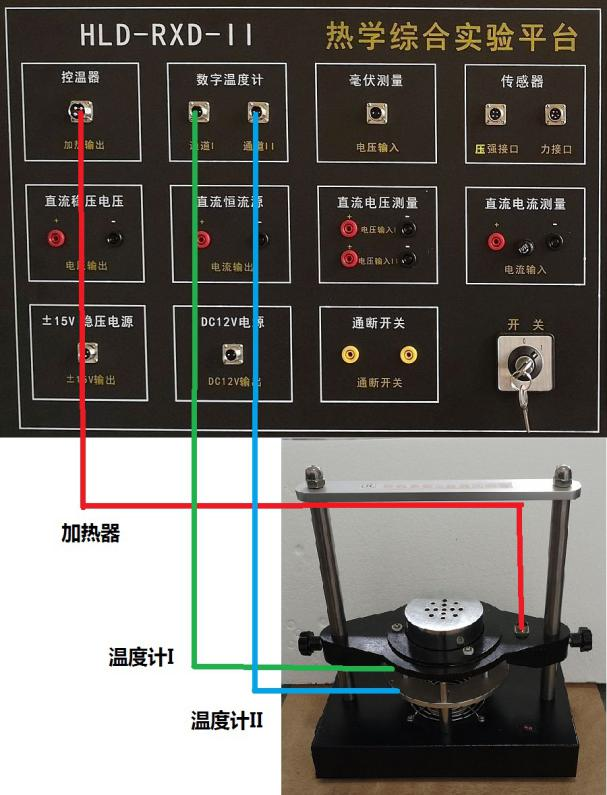
\includegraphics[width=\linewidth]{assets/image1.jpeg}
    \caption{导热系数实验接线与装置示意}
  \end{minipage}
\end{figure}

实验所用主要器材包括热学综合实验平台、导热系数实验附件、加热盘、散热盘、硅橡胶样品、两路数字温度计及计时模块。

\section{实验原理}

\subsection{热传导定律}
当物体内部存在温度差时，热量会从高温区域向低温区域传递，这种现象称为热传导。若热量沿垂直于样品表面的方向传输，则傅里叶热传导定律可写为
\[
  \frac{\mathrm{d}Q}{\mathrm{d}t}
  =
  -\lambda S \frac{\mathrm{d}T}{\mathrm{d}z},
\]
其中 $\lambda$ 为材料的导热系数，$S$ 为垂直于传热方向的截面积，负号表示热流方向与温度升高方向相反。

\subsection{稳态法测量导热系数}
将待测硅橡胶样品 $B$ 夹在加热盘 $A$ 与散热盘 $P$ 之间。稳定加热后，上下两盘分别维持近似恒定温度 $T_1$ 与 $T_2$，样品内部便建立起沿厚度方向的稳定温度梯度。若样品厚度为 $h_B$、半径为 $R_B$，且满足 $h_B \ll 2R_B$，则可近似认为热量只沿轴向传递，此时
\[
  \frac{\mathrm{d}T}{\mathrm{d}z}
  \approx
  \frac{T_1 - T_2}{h_B}.
\]

稳态时，加热盘传给样品的热流率等于样品传给散热盘的热流率，也等于散热盘向环境散失的热流率。因此只要求出散热盘在稳态温度 $T_2$ 附近的散热速率，就能间接得到样品中的传热速率。

\subsection{散热速率的参量转换}
设散热盘质量为 $m$，比热容为 $c$，其温度在自然冷却过程中随时间变化为 $T(t)$。若取冷却曲线在 $T=T_2$ 附近的切线斜率，则散热盘在该温度下的散热速率可写为
\[
  \left.\frac{\mathrm{d}Q}{\mathrm{d}t}\right|_{T=T_2}
  =
  -mc
  \left.\frac{\mathrm{d}T}{\mathrm{d}t}\right|_{T=T_2}.
\]
考虑到自然冷却时散热盘全部表面都暴露于空气中，而稳态传热时其上表面被样品覆盖，因此需要按有效散热面积进行修正。若散热盘半径和厚度分别为 $R_P$ 与 $h_P$，则修正后的散热速率为
\[
  \frac{\mathrm{d}Q}{\mathrm{d}t}
  =
  -mc
  \frac{R_P + 2h_P}{2R_P + 2h_P}
  \left.\frac{\mathrm{d}T}{\mathrm{d}t}\right|_{T=T_2}.
\]

再由
\[
  \frac{\mathrm{d}Q}{\mathrm{d}t}
  =
  \lambda \pi R_B^2 \frac{T_1 - T_2}{h_B},
\]
即可得到待测样品导热系数的计算式
\[
  \lambda
  =
  -mc
  \frac{R_P + 2h_P}{2R_P + 2h_P}
  \frac{h_B}{\pi R_B^2 (T_1 - T_2)}
  \left.\frac{\mathrm{d}T}{\mathrm{d}t}\right|_{T=T_2}.
\]
本实验中铜盘比热容取
\[
  c = 0.385 \times 10^3\ \mathrm{J\,kg^{-1}\,^{\circ}C^{-1}}.
\]

\begin{figure}[htbp]
  \centering
  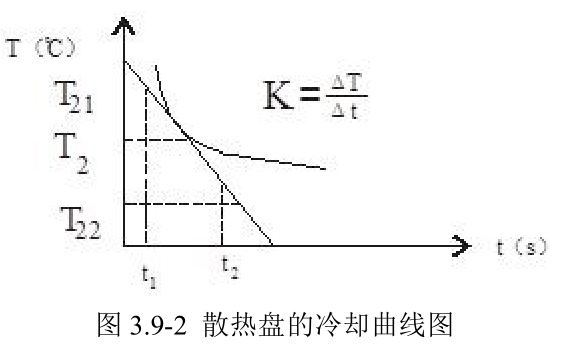
\includegraphics[width=0.58\linewidth]{assets/散热盘冷却曲线示意图.png}
  \caption{散热盘在稳态温度附近的冷却曲线示意图}
\end{figure}

\section{实验内容和步骤}

\noindent\textbf{1.} 按照实验接线图连接装置，打开热学综合实验平台电源，在实验目录中选择“非良导体导热系数实验”，并拖出温度计 I、温度计 II 和计时器模块。

\begin{figure}[htbp]
  \centering
  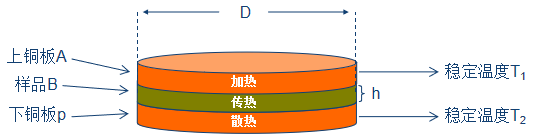
\includegraphics[width=0.86\linewidth]{assets/image9.png}
\end{figure}

\noindent\textbf{2.} 记录样品和散热盘的几何参数，包括硅橡胶样品厚度 $h_B$、半径 $R_B$，散热盘厚度 $h_P$（仪器软件中分别记为 $R_A$ 和 $h_A$）、半径 $R_P$ 以及散热盘质量 $m$。

\noindent\textbf{3.} 将硅橡胶样品夹在加热盘 A 与散热盘 P 之间，调节支架上的微调螺丝，使样品 B 与上下铜盘 A、P 接触良好；将两支温度探头分别插入对应铜盘侧孔并与铜盘充分接触。A 为温度通道 I，B 为温度通道 II。

\noindent\textbf{4.} 设置控温器温度为 $80\,^{\circ}\mathrm{C}$，启动温度记录功能，系统每隔 $60\,\mathrm{s}$ 自动记录一次加热盘温度 $T_1$ 与散热盘温度 $T_2$。

\noindent\textbf{5.} 待加热一段时间后（约40分钟），当 $T_1$ 读数基本稳定（波动小于0.2℃），再每隔 $2\,\mathrm{min}$ 记录一次 $T_1$ 和 $T_2$ 于表 \ref{table:steady}，直到 $T_2$ 也基本稳定（10分钟内波动小于0.2）。

\noindent\textbf{6.} 测量散热盘在稳态温度 $T_2$ 附近的散热速率：移开A，取下B，再使P与A直接接触，当P的温度上升到高于稳态 $T_2$ 的值约10℃左右时，再将A移开，让P的所有表面均暴露于空气中。使P自然冷却，并开始记录散热温度与时间入表 \ref{table:cooling} 中，直到温度下降到$T_2$以下一定值，停止记录。

\noindent\textbf{7.} 根据冷却曲线在 $T=T_2$ 附近的切线斜率求出冷却速率，再代入导热系数公式，计算样品的导热系数。

\newcolumntype{Y}{>{\centering\arraybackslash}X}

\begin{LabRecordTable}
  \centering
  \caption{参数记录表}
  \label{table:param}
  \renewcommand{\arraystretch}{1.25}
  \begin{tabularx}{\textwidth}{*{5}{Y}}
    \toprule
    散热盘厚度 $h_P$/mm & 样品厚度 $h_B$/mm & 散热盘半径 $R_P$/mm & 样品半径 $R_B$/mm & 散热盘质量 $m$/g \\
    \midrule
    \rule{0pt}{2.8ex} & & & & \\
    \bottomrule
  \end{tabularx}
\end{LabRecordTable}

\begin{LabRecordTable}
  \centering
  \caption{稳态测温记录表}
  \label{table:steady}
  \renewcommand{\arraystretch}{1.25}
  \setlength{\tabcolsep}{3.5pt}
  \begin{tabularx}{\textwidth}{c *{10}{Y}}
    \toprule
    序号 $i$ & 1 & 2 & 3 & 4 & 5 & 6 & 7 & 8 & 9 & 10 \\
    \midrule
    $T_1$/\si{\celsius} & & & & & & & & & & \\
    $T_2$/\si{\celsius} & & & & & & & & & & \\
    \bottomrule
  \end{tabularx}
\end{LabRecordTable}

\begin{LabRecordTable}
  \centering
  \caption{散热盘自然冷却记录表}
  \label{table:cooling}
  \renewcommand{\arraystretch}{1.25}
  \setlength{\tabcolsep}{3.5pt}
  \begin{tabularx}{\textwidth}{c *{10}{Y}}
    \toprule
    $t$/s & 30 & 60 & 90 & 120 & 150 & 180 & 210 & 240 & 270 & 300 \\
    \midrule
    $T_2$/\si{\celsius} & & & & & & & & & & \\
    \midrule
    $t$/s & 330 & 360 & 390 & 420 & 450 & 480 & 510 & 540 & 570 & 600 \\
    \midrule
    $T_2$/\si{\celsius} & & & & & & & & & & \\
    \bottomrule
  \end{tabularx}
\end{LabRecordTable}

\section{数据处理}
\begin{enumerate}[label=\arabic*. ]
  \item 由表 \ref{table:steady} 中的数据求加热盘与散热盘的稳态温度 $T_1$、$T_2$；如有需要，可先进行离群值检查后再取平均值。
  \item 由表 \ref{table:cooling} 中数据作散热盘的 $T$-$t$ 冷却曲线，在 $T=T_2$ 附近取切线，求出冷却速率 $\left.\frac{\mathrm{d}T}{\mathrm{d}t}\right|_{T=T_2}$。
  \item 将 $m$、$R_P$、$h_P$、$R_B$、$h_B$、$T_1$、$T_2$ 及冷却速率代入导热系数公式，计算样品导热系数 $\lambda$。
  \item 完成阶段可根据计算结果与材料常见导热系数范围进行比较，并结合稳态建立情况、接触热阻、环境散热和斜率读取误差讨论实验偏差来源。
\end{enumerate}

\section{实验的分析和总结}
完成阶段补充以下内容：
\begin{enumerate}[label=\arabic*. ]
  \item 根据实测数据给出导热系数计算结果，并说明其物理意义；
  \item 结合稳态法和参量转换法，分析本实验设计的关键思路；
  \item 讨论样品与铜盘接触情况、温度稳定程度、环境散热和冷却曲线斜率选取对结果的影响。
\end{enumerate}

\insertRawDataPage

\end{document}
